\documentclass[12pt,letterpaper]{article}
\usepackage{graphicx,textcomp}
\usepackage{natbib}
\usepackage{setspace}
\usepackage{fullpage}
\usepackage{color}
\usepackage[reqno]{amsmath}
\usepackage{amsthm}
\usepackage{fancyvrb}
\usepackage{amssymb,enumerate}
\usepackage[all]{xy}
\usepackage{endnotes}
\usepackage{lscape}
\newtheorem{com}{Comment}
\usepackage{float}
\usepackage{hyperref}
\newtheorem{lem} {Lemma}
\newtheorem{prop}{Proposition}
\newtheorem{thm}{Theorem}
\newtheorem{defn}{Definition}
\newtheorem{cor}{Corollary}
\newtheorem{obs}{Observation}
\usepackage[compact]{titlesec}
\usepackage{dcolumn}
\usepackage{tikz}
\usetikzlibrary{arrows}
\usepackage{multirow}
\usepackage{xcolor}
\newcolumntype{.}{D{.}{.}{-1}}
\newcolumntype{d}[1]{D{.}{.}{#1}}
\definecolor{light-gray}{gray}{0.65}
\usepackage{url}
\usepackage{listings}
\usepackage{color}

\definecolor{codegreen}{rgb}{0,0.6,0}
\definecolor{codegray}{rgb}{0.5,0.5,0.5}
\definecolor{codepurple}{rgb}{0.58,0,0.82}
\definecolor{backcolour}{rgb}{0.95,0.95,0.92}

\lstdefinestyle{mystyle}{
	backgroundcolor=\color{backcolour},   
	commentstyle=\color{codegreen},
	keywordstyle=\color{magenta},
	numberstyle=\tiny\color{codegray},
	stringstyle=\color{codepurple},
	basicstyle=\footnotesize,
	breakatwhitespace=false,         
	breaklines=true,                 
	captionpos=b,                    
	keepspaces=true,                 
	numbers=left,                    
	numbersep=5pt,                  
	showspaces=false,                
	showstringspaces=false,
	showtabs=false,                  
	tabsize=2
}
\lstset{style=mystyle}
\newcommand{\Sref}[1]{Section~\ref{#1}}
\newtheorem{hyp}{Hypothesis}

\title{Problem Set 4}
\date{Due: April 4, 2022}
\author{Applied Stats II}


\begin{document}
	\maketitle
	\section*{Instructions}
	\begin{itemize}
		\item Please show your work! You may lose points by simply writing in the answer. If the problem requires you to execute commands in \texttt{R}, please include the code you used to get your answers. Please also include the \texttt{.R} file that contains your code. If you are not sure if work needs to be shown for a particular problem, please ask.
		\item Your homework should be submitted electronically on GitHub in \texttt{.pdf} form.
		\item This problem set is due before class on Monday April 4, 2022. No late assignments will be accepted.
		\item Total available points for this homework is 80.
	\end{itemize}

	\vspace{.25cm}
\section*{Question 1}
\vspace{.25cm}
\noindent We're interested in modeling the historical causes of infant mortality. We have data from 5641 first-born in seven Swedish parishes 1820-1895. Using the "infants" dataset in the \texttt{eha} library, fit a Cox Proportional Hazard model using mother's age and infant's gender as covariates. Present and interpret the output.


\section*{Question 1 - My Answer} 


\begin{lstlisting}[language=R]

# Load infants dataset
data(infants)

# using Tutorial 10 as reference, where 'child' was used
infant_survivor <- with(infants, Surv(enter, exit, event))

# using survit to create the survival model

## and need to run a Cox Proportional Hazard regression on the data

km <- survfit(infant_survivor ~ 1, data = infants)


# summary(km, times = seq(0, 15, 1))
# event = 0, exit = 365, exit = 5 

summary(km, times = seq(0, 365, 5))
autoplot(km, main="Overall Infant Survival Rate",
         xlab = "Time",
         ylab = "Survival Rate")


\end{lstlisting}


\begin{figure}
  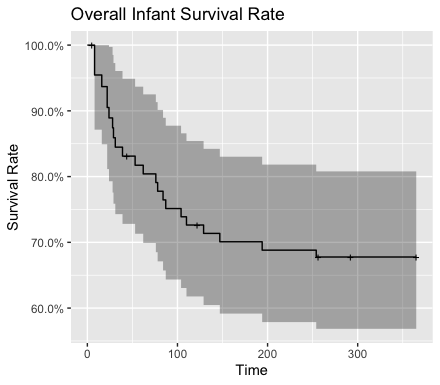
\includegraphics[width=\textwidth]{Rplot.png}
\end{figure}






\begin{lstlisting}[language=R]


# Run a Cox Proportional Hazard Regression
# referencing tutorial 10
cox <- coxph(Surv(enter, exit, event) ~ sex + age, data = infants)
summary(cox)
drop1(cox, test = "Chisq")
# stargazer(cox, type = "text")
stargazer(cox)

## For the Survival Rate in the first 100 days there is an increase, which then decrease after 
## 100 days but the overall infant survival rate is shown to be quite low. 


\end{lstlisting}


\begin{table}[!htbp] \centering 
  \caption{Cox Proportional Hazard Regression} 
  \label{} 
\begin{tabular}{@{\extracolsep{5pt}}lc} 
\\[-1.8ex]\hline 
\hline \\[-1.8ex] 
 & \multicolumn{1}{c}{\textit{Dependent variable:}} \\ 
\cline{2-2} 
\\[-1.8ex] & enter \\ 
\hline \\[-1.8ex] 
 sexboy & $-$0.485 \\ 
  & (0.442) \\ 
  & \\ 
 age & $-$0.040 \\ 
  & (0.045) \\ 
  & \\ 
\hline \\[-1.8ex] 
Observations & 105 \\ 
R$^{2}$ & 0.019 \\ 
Max. Possible R$^{2}$ & 0.800 \\ 
Log Likelihood & $-$83.626 \\ 
Wald Test & 2.000 (df = 2) \\ 
LR Test & 1.992 (df = 2) \\ 
Score (Logrank) Test & 2.034 (df = 2) \\ 
\hline 
\hline \\[-1.8ex] 
\textit{Note:}  & \multicolumn{1}{r}{$^{*}$p$<$0.1; $^{**}$p$<$0.05; $^{***}$p$<$0.01} \\ 
\end{tabular} 
\end{table} 




\end{document}
